\documentclass[a4paper,12pt]{article}
\usepackage{syntax}
\usepackage{amsmath}
\usepackage{algorithm}
\usepackage[noend]{algpseudocode}
\usepackage{pgfplots}
\usepackage{listings}
\usepackage[nottoc]{tocbibind}
\setlength{\parindent}{4em} 
\usepackage{graphicx}
\graphicspath{ {images/} }
%paragraph spacing
\setlength{\parskip}{1em}

%Line spacing
\renewcommand{\baselinestretch}{1.5}
\title{A1}
\author{Kevin R. Clemmons}
\date{October 2015}

\begin{document}

\maketitle
\newpage 
%
\section{Curl Demonstration}
For the curl assignment, I used the aviation digital weather service to acquire a METAR for Norfolk International Airport which has the ICAO Code: KORF. The following curl command was used: \\
curl -d ``ids=korf&format=raw&data=0&hors=0'' ``https://www.aviationweather.gov/metar/data'' $>$ resul.html
\subsection{Form Before }
\begin{figure}[h]
\centering
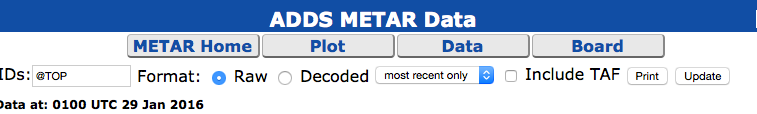
\includegraphics[width=14cm]{FormBefore}
\end{figure}
\subsection{Form After}
\begin{figure}[h]
\centering
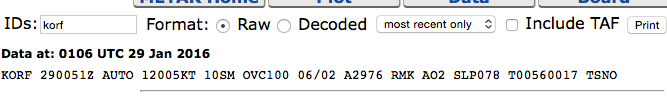
\includegraphics[width=14cm]{FormAfterCurlCommand}
\end{figure}
The html file for the result of the curl command is located in the folder called curl
\newpage 
%%-------------------------------------------------------
%
\section{PDF Link Extractor} 
\subsection{Libraries Used}
\begin{itemize}
    \item urllib2
    \item urllib
    \item urlparse
    \item sys 
    \item httplib
    \item errno
    \item socket
    \item bs4 
\end{itemize}


\subsection{Compilation}
\begin{itemize}
    \item Not Needed
\end{itemize}
\subsection{Running}
\begin{itemize}
    \item \verb To run, enter the command: python pdfLinks.py <url-name>
\end{itemize}
\subsecton{Notes}
\subsubsection{This program was tested with the following links}
\begin{itemize}
\item \verb http://ocw.mit.edu/courses/electrical-engineering-and-computer-science/ \\ \verb 6-088-introduction-to-c \\ \verb -memory-management-and-c-object-oriented-programming- january-\verb iap-2010/lecture-notes/

\item  \verb http://www.cs.toronto.edu/~suzanne/publications.html

\item \verb http://www.cs.odu.edu/~mln/teaching/cs532-s16/test/pdfs.html

\item \verb http://www.cs.odu.edu/~mln/

\item \verb http://www.macs.hw.ac.uk/~jim/112MH1/tuts/
\end{itemize}
If you would like a demonstration of the test cases, enter the command \verb python pdfLinks.py -d \\ 
A captured output of the above test cases is located in the file called results.txt, which can be found in the pdfLinks folder. 



\subsubsection{Sources}
\begin{itemize}
    \item Exception handling in lines 42-45
    \begin{itemize}
        \item 	url: http://stackoverflow.com/questions/20568216/python-handling-socket-error-errno-104-connection-reset-by-peer
        \item Accessed: 1/28/15
    \end{itemize}
	
	\item Exception handline for requests
	\begin{itemize}
	    \item url: http://stackoverflow.com/questions/666022/what-errors-exceptions-do-i-need-to-handle-with-urllib2-request-urlopen
		\item Accessed: 1/24/15
	\end{itemize}
		
			
	\item Handling link-redirections in line 62-77
	\begin{itemize}
	    \item url: http://www.zacwitte.com/resolving-http-redirects-in-python
	    \item Accessed: 1/28/15
	\end{itemize}
		

	\item Handling incomplete links in line 152-153
	\begin{itemize}
	    \item url: http://stackoverflow.com/questions/27397990/python-parsing-html-for-complete-links-urls
	    \item * Accessed: 1/28/15
	\end{itemize}
	
\end{itemize}
\newpage 
\section{Graph}
The graph below was generated by creating an adjacency matrix as seen below. \\
\begin{figure}[h]
\centering
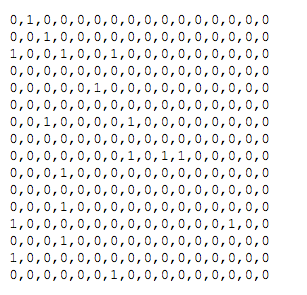
\includegraphics[width=5cm]{adjacencyMatrix}
\end{figure}

Once the matrix was created, the graph below was created from the following website: http://graphonline.ru/en/ \\ 
\begin{figure}[h]
\centering
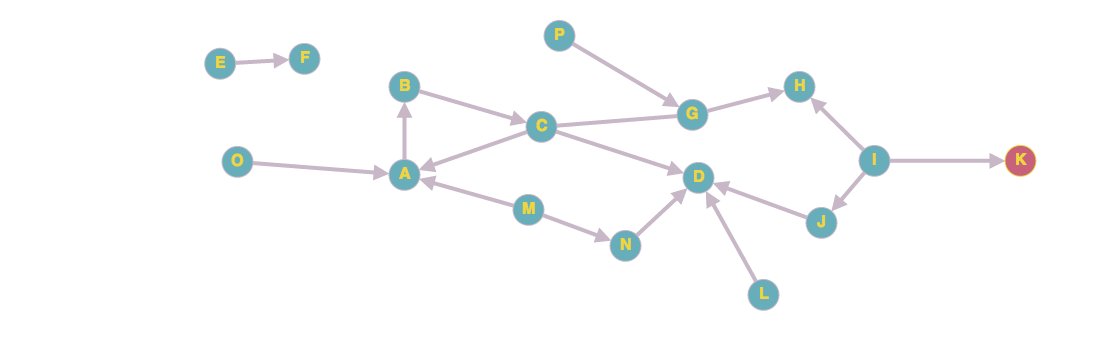
\includegraphics[width=20cm]{graph}
\end{figure}
\newpage 
\subsection{Values for the Graph}
The following vertexes make up the components of the graph.
\begin{itemize}
    \item IN: O, P, L
    \item SCC: C
    \item OUT: K,H,G
    \item Tendrils: M
    \item Tubes: B,C,G,H
    \item Disconnected: E,I
\end{itemize}
\end{document}
